\documentclass[conference]{IEEEtran}
\IEEEoverridecommandlockouts

\usepackage{cite}
\usepackage{amsmath,amssymb}
\usepackage{graphicx}
\usepackage{booktabs}
\usepackage{url}
\usepackage{xcolor}
\usepackage[hidelinks]{hyperref}

% Default float parameters make LaTeX defer floats aggressively; with five
% figures plus a full-width table they all pile up at the end, leaving pages
% two-thirds empty. Allowing more float area per page packs them next to the
% text that references them.
\renewcommand{\topfraction}{0.92}
\renewcommand{\bottomfraction}{0.8}
\renewcommand{\textfraction}{0.06}
\renewcommand{\floatpagefraction}{0.8}
\setcounter{topnumber}{3}
\setcounter{totalnumber}{4}

\newcommand{\tierone}[1]{#1}

\begin{document}

\title{Solver-Verified Text-Conditioned Sokoban Level Generation:\\
Autoregressive Models Can Count, One-Shot Decoders Cannot}

\author{\IEEEauthorblockN{Aayush Kumar Tiwari}
\IEEEauthorblockA{\textit{KJ Somaiya School of Engineering} \\
aayushkumar345@gmail.com}
\and
\IEEEauthorblockN{Prateeksha Kini}
\IEEEauthorblockA{\textit{KJ Somaiya School of Engineering}}}

\maketitle

\begin{abstract}
We compare three generative model families on text-conditioned Sokoban level
generation and evaluate them with an exhaustive A* solver rather than a learned
or heuristic proxy. Because the state space of a $10\times10$ Sokoban level is
bounded and every prune we use is sound, exhausting the search is a
\emph{proof} of unsolvability: the verifier is a decision procedure, not a
one-sided test. We therefore report three outcomes (solved, proven
unsolvable, and timed out) rather than two. Our central finding is that
autoregressive generation satisfies hard counting constraints that one-shot
generators cannot: a $10.7$M-parameter decoder-only transformer emitting a level
cell by cell reaches $82.6\%$ structural validity unaided, while a conditional
VAE decoding all $100$ cells from a latent vector produces \textbf{zero} valid
levels in $100{,}000$ draws under argmax decoding, because the argmax of a
product of independent per-cell marginals annihilates exactly the rare tiles the
constraints are about. Constrained decoding closes the counting gap
deterministically, at $100\%$ validity. Solvability, however, does not follow
from validity: an empty-room baseline with no interior walls is solvable
$23.4\%$ of the time against the transformer's $49.6\%$, so the gap is real but
solvability alone is not a sufficient objective: a retrieval baseline that
copies training levels maximises it at zero novelty. Two results cut against the
simple story: repairing the VAE's counting errors yields $76.6\%$ solvability,
\emph{above} the transformer, locating the autoregressive advantage in counting
rather than in spatial structure; and every family fails to extrapolate,
producing $\sim\!30$-move levels when asked for $\sim\!116$. Measuring across
three training seeds per configuration rather than one turns out to be
essential: solvability moves by $\pm 7$ points across seeds while validation
loss moves by $\pm 0.005$. We argue the results table must be read as a joint constraint over
solvability, difficulty control and novelty. This work replicates and extends
Todd et al.~\cite{todd2023level}; the data-scaling and tokenization findings are
theirs, and we claim neither.
\end{abstract}

\begin{IEEEkeywords}
procedural content generation, generative models, constrained decoding,
verification, Sokoban
\end{IEEEkeywords}

\section{Introduction}

Evaluating a generative model is usually a matter of proxies. Perplexity does
not tell you whether a program runs; a discriminator score does not tell you
whether a level can be finished. The situation is better than it is sometimes
described, since HumanEval executes unit tests~\cite{chen2021codex}, Lean checks
proofs~\cite{demoura2021lean}, and text-to-SQL is scored by execution
accuracy~\cite{yu2018spider}, so it is simply false that no metric can tell
you whether a generated artifact works.

What those verifiers share is that they are \emph{sound but incomplete}. A unit
test that passes does not prove a program correct, and a test suite cannot prove
a program wrong: it can only fail to find a witness. The verifier answers "yes"
reliably and "no" only provisionally.

Sokoban is unusual in admitting the other kind of verifier. The state space of a
$10\times10$ level with four boxes is finite and small enough to exhaust. Given
pruning rules that are \emph{sound}, meaning they discard only states from which
no solution exists, running the open set to empty is a constructive proof that
no solution exists. The verifier is a \textbf{decision procedure}. This is why
we report a three-way outcome; collapsing "timed out" into "unsolvable" would
convert an absence of evidence into a false proof, in a direction that
flatters the numbers.

The second question we ask is about model architecture. A valid level needs
\emph{exactly} one player, four boxes and four goals. A transformer that emits
one cell at a time conditions each decision on how many boxes it has already
placed; a VAE or GAN decoder that emits all $100$ cells from a single latent
vector cannot, because its per-cell outputs are conditionally independent given
the latent. This is a structural prediction about which family can satisfy a
counting constraint, and an exhaustive solver lets us measure both whether the
constraint is met and whether the resulting level is any good.

\paragraph{Contributions}
\begin{enumerate}
\item An exhaustive, validated A* Sokoban solver used as a decision procedure,
      with a soundness ablation and a node-cap convergence curve
      (Section~\ref{sec:solver}).
\item A three-family comparison (from-scratch transformer, conditional VAE,
      conditional GAN) at roughly comparable parameter counts, with
      constrained decoding and repair reported as separate rows so that
      \emph{counting} and \emph{spatial understanding} are measured separately
      (Sections~\ref{sec:method},~\ref{sec:results}).
\item Baselines that constrain the interpretation of the headline number: an
      open-room baseline that shows solvability is easy to obtain, and a
      retrieval baseline that shows it is trivially maximised by copying.
\item Data-quality findings about the standard Boxoban A* solution set that
      affect anyone using it for supervision (Section~\ref{sec:dataset}).
\end{enumerate}

We are explicit about provenance throughout. Claims are marked as
\textbf{Tier 1} (proven by our experiments), \textbf{Tier 2} (justified by
citation) or \textbf{Tier 3} (admitted defaults, such as untuned
hyperparameters).

\section{Related Work}

\paragraph{LLMs for level generation}
Todd et al.~\cite{todd2023level} fine-tune GPT-2 variants to generate Sokoban
levels from a character encoding and study how solvability scales with training
data and with tokenization. This paper is a replication and extension of that
work; \textbf{the data-scaling result, the solvability-versus-conditioning
setup, and the tokenization finding are theirs}, and we claim none of them.
MarioGPT~\cite{sudhakaran2023mariogpt} conditions level generation on natural
language for Super Mario Bros., where playability is checked by an $A^*$ agent
that is a sound but incomplete verifier: it can confirm a level is playable
but cannot prove one is not.

\paragraph{Our delta}
Relative to~\cite{todd2023level} we add three things: constrained decoding with
feasibility forcing that makes structural validity deterministic rather than
learned; three-way solver reporting that distinguishes proven unsolvability from
timeout; and a controlled multi-family comparison at comparable parameter
counts, including one-shot decoders and non-learned baselines.

\paragraph{PCGML}
Procedural content generation via machine learning~\cite{summerville2018pcgml}
has long used autoencoders and GANs over tile grids. Our contribution is not a
new architecture but a verification methodology: the same tile-grid models,
judged by a decision procedure instead of a proxy.

\paragraph{Sokoban and search}
Sokoban is PSPACE-complete in general~\cite{culberson1997sokoban}, and the
solver literature is built on domain-specific pruning~\cite{junghanns2001sokoban}.
Our solver is deliberately conservative: only two prunes, both sound, because an
unsound prune produces false proofs of unsolvability. The Boxoban
corpus~\cite{boxobanlevels} was introduced for model-free planning research and
generated by the procedure of Racani\`ere et al.~\cite{racaniere2017imagination};
its test split is the one used by Orseau et al.~\cite{orseau2018single}.

\section{Dataset}
\label{sec:dataset}

We use the Boxoban \texttt{unfiltered} split~\cite{boxobanlevels}: $100{,}000$
training levels, $5{,}000$ from the \emph{official} validation split (we do not
carve a validation set out of train), and the $1{,}000$-level test split held
frozen for solver validation and as the real-level ceiling row. Solution lengths
come from the A* solution set of Garriga-Alonso et
al.~\cite{garrigaalonso2024planning}.

\subsection{Verified format properties}
We verified rather than assumed every property the representation depends on
(Tier 1). Over $50$ level files the tile alphabet is exactly
$\{\texttt{\#}, \texttt{@}, \texttt{\$}, \texttt{.}, \texttt{\textvisiblespace}\}$;
in particular \textbf{neither \texttt{*} (box on goal) nor \texttt{+} (player on
goal) occurs anywhere}, so a box never \emph{starts} on a goal. That single fact
is what makes the five-channel tensor, the six-symbol vocabulary and the
"exactly four \texttt{\$} and four \texttt{.}" constraint well-defined; had it
failed, each would have broken silently. Over $10{,}000$ levels every grid is
$10\times10$ with a complete wall border and exactly one player, four boxes and
four goals, with zero violations, and there are zero collisions between train
and either held-out split. Files use CRLF endings, which the parser
normalises.

\subsection{Solution lengths count moves, not pushes}
The solution set stores an action string over $\{0,1,2,3\}$ = Up, Right, Down,
Left, and a \texttt{Steps} field equal to its length. \texttt{Steps} therefore
counts \textbf{player moves, not pushes} (Tier 1). We confirmed the action
encoding by replaying: under this convention the actions reach the goal state
exactly, and no other permutation of the four directions, with or without
transposition, replays even one of the levels that fail. Their search minimised
moves, so \texttt{Steps} is move-optimal where it is valid. This distinction
sets the units of every caption and of the controllability metric.

\subsection{A data-quality finding}
The solution set documents rows whose action field is
\texttt{SEARCH\_STATE\_FAILED} or \texttt{NOT\_FOUND}. We additionally found rows
that \emph{look} well-formed, a plain digit string, but \textbf{do not
replay to a solved state}: $63/1000$ ($6.3\%$) of \texttt{unfiltered\_test} and
approximately $0.7\%$ of \texttt{unfiltered\_train}. They fail by walking into a
wall or making an impossible push part-way through, and treating blocked moves
as no-ops does not rescue any of them. We therefore \textbf{replay-validate
every solution} and drop levels whose solution does not replay ($0.73\%$ of
train, $7.4\%$ of validation and test). Anyone using this set for supervision
should do the same; a caption built on a wrong length is worse than no example.

\subsection{Captions}
Five features are computed from the grid; nothing is hand-labelled. Difficulty
is the solution length binned by the terciles of the training distribution
($\leq26$, $\leq35$, $>35$ moves); solution length is quoted to the nearest five
moves; wall density is the interior wall fraction split at the training median
($0.500$); connectivity is the mean number of non-wall neighbours per floor cell
split at the training median ($2.889$); and box clustering is the mean pairwise
Manhattan distance between boxes split at the training median ($3.500$). A
caption reads, for example, \texttt{"hard, \textasciitilde40 moves, dense walls,
corridors, boxes scattered"}.

The connectivity feature was chosen empirically. The natural first choice,
counting connected floor components, is \textbf{constant} on this corpus:
measured over $20{,}000$ training levels every Boxoban level has exactly one
connected floor region, so the feature carries no information and cannot bin
anything. We use mean floor degree instead, which ranges $2.19$ to $3.36$.

The same five features are encoded twice: as caption text for the transformer,
and as a $10$-dimensional vector for the VAE and GAN. \textbf{These are different
information channels}, so the family comparison is not perfectly controlled on
conditioning; we state this rather than claim otherwise.

\section{Method}
\label{sec:method}

\subsection{Transformer (primary)}
A decoder-only transformer written from scratch: $d_{\text{model}}=384$, $6$
layers, $6$ heads, $d_{\text{ff}}=1536$, learned positional embeddings,
pre-norm, GELU, dropout $0.1$, tied input/output embeddings, for $10{,}734{,}336$
parameters. We deliberately do \emph{not} use a fine-tuned pretrained model as
the primary system, so that the family comparison is roughly parameter-fair
($10.7$M against $1.1$M and $1.1$M) rather than $82$M against $1$M. The
vocabulary is $48$ hand-written characters; the sequence is
\texttt{<bos>} caption \texttt{<sep>} grid($110$ chars) \texttt{<eos>}, and the
loss is masked over the caption prefix so the model is trained to predict the
grid, not the caption.

\subsection{Constrained decoding}
\label{sec:constrained}
A manual sampling loop applies a per-step logit mask. Border cells are forced to
wall; the eleventh character of each row is forced to newline; and any tile whose
quota is exhausted is masked. The rule that matters is \textbf{feasibility
forcing}: letting $r=(1-n_{\text{player}})+(4-n_{\text{box}})+(4-n_{\text{goal}})$
be the specials still owed and $\ell$ the interior cells remaining, when
$\ell \leq r$ we mask \texttt{\#} and space so that only specials can be emitted.
Masking upper bounds alone enforces "at most four boxes", not "exactly four".
With nine specials in $64$ interior cells this rule rarely binds, which is
precisely the trap: an implementation without it looks correct on a handful of
samples and fails in the tail.

We instrument the rule and report the \textbf{forced-token rate}, which is a free
measure of how well the model learned to count unaided.

\subsection{Conditional VAE}
An MLP encoder and decoder over a $5\times10\times10$ one-hot tensor, latent
dimension $32$, $1{,}098{,}292$ parameters. MLPs rather than convolutions:
$10\times10$ does not factor cleanly for strided convolutions and at $100$ cells
convolutions buy nothing while costing shape bugs. The reconstruction loss is
\textbf{per-cell categorical cross-entropy over the channel dimension}, not MSE,
which treats a categorical axis as a metric space and is a common wrong default.
Posterior collapse is prevented with free bits~\cite{kingma2016freebits} at a
$0.05$-nat floor.

We report \textbf{two decoding protocols, both mandatory}. Under argmax, floor
or wall wins almost everywhere, because the argmax of a product of marginals is
not the mode of the joint and rare tiles are exactly what gets annihilated.
Reporting argmax alone would be an unfair protocol, so we also report per-cell
sampling, which preserves marginal tile rates and gives roughly the right
\emph{number} of boxes in the wrong \emph{places}.

\subsection{Conditional GAN}
An MLP generator and discriminator, $1{,}082{,}357$ parameters combined, with
straight-through Gumbel-softmax~\cite{jang2017gumbel} discretisation annealed
from temperature $1.0$ to $0.3$, and one-sided label smoothing. Training on
continuous logits and taking argmax only at sampling time is not a valid option:
the discriminator can then separate real one-hot tensors from soft generator
output purely by per-cell entropy, training collapses to that trivial
discriminator, and the generator learns nothing about layout. This family was
hard time-boxed; mode collapse is reported as a finding, not treated as a
failure to fix.

\subsection{Repair}
Any structurally invalid grid is projected onto the nearest valid grid using the
model's own predicted probabilities: the border is forced to wall, excess boxes,
goals and players are dropped lowest-probability first, deficits are filled
highest-probability first, and specials are never placed on the border. Repair is
idempotent and is the identity on already-valid grids. Reporting post-repair
solvability decomposes the comparison into two separable questions: \emph{can the
model count?} (structural validity) and \emph{does it understand spatial
structure?} (post-repair solvability). Without it a reader cannot tell whether
the GAN is bad at Sokoban or merely bad at arithmetic.

\subsection{Baselines}
Random placement (uniform interior walls at the training-median density, then
random specials) is the floor. \textbf{Open room}, border walls only, can
invalidate the headline number, since an empty room has no interior walls to
freeze a box against. Rule-based generation adds a floor-connectivity check and
places boxes and goals only on live squares. \textbf{Retrieval} samples a
training level verbatim, making the complementary point that solvability alone is
maximised by copying. Held-out Boxoban levels give the ceiling row.

\subsection{Comparison protocol}
The transformer is reported \textbf{both with and without} constrained decoding,
so a reader can compare unconstrained-to-unconstrained across all three
families and see the constrained result separately. Structural validity and
solvability are never merged into one number: merging them compares decoding
schemes rather than model families.

\section{Solver}
\label{sec:solver}

\subsection{Design}
Levels are represented as integer bitmasks (walls, goals, boxes) plus a player
cell index. Successors are \textbf{pushes}, not single steps. For hashing, the
player's exact cell is irrelevant and only its reachable region matters, so
the state key is (minimum reachable cell, box mask). Without this
canonicalisation, states differing only by player position within one region are
distinct and the search inflates by roughly the region size; measured on the
$1{,}000$ real test levels, the starting region averages $19.1$ cells (median
$22.5$, maximum $46$).

The heuristic precomputes, per goal, a backward BFS map of the minimum pushes to
bring a box to that goal, ignoring other boxes but respecting walls, and takes
the minimum-cost assignment of boxes to goals~\cite{kuhn1955hungarian}. It is
admissible, since each push moves one box one cell, and strictly tighter than
sum-of-Manhattan because it respects walls.

\subsection{Two sound prunes, and nothing else}
A cell is \emph{dead} if a box there can reach no goal under the relaxation
above; any box on a dead square is a proven deadlock, which subsumes corner
deadlocks. A box is \emph{frozen} if it is blocked along both axes, where a
blocker is a wall, a dead square, or another frozen box, with a
currently-evaluated box treated as blocking to terminate the recursion; any
frozen box off a goal is a proven deadlock. We admit nothing heuristic:
\textbf{an unsound prune produces false proofs of unsolvability}, which is the
worst failure mode available here because it corrupts the headline number
invisibly and in a plausible direction.

\texttt{unsolvable} is returned \textbf{only} when the open set empties before
any budget is hit. Every cap hit is \texttt{timeout}.

\subsection{Validation}
On all $1{,}000$ real test levels the solver achieves a \textbf{100.00\% solve
rate} with zero \texttt{unsolvable} verdicts and zero timeouts (Tier 1), and
every returned solution replays to a solved state under an independent
simulator. Against the published solutions our push-optimal length is $\leq$
theirs on $926/926$ comparable levels and our reconstructed move length is
$\geq$ their move-optimal length on $926/926$, both as theory requires.

The \textbf{soundness ablation} reruns a $200$-level sample with both prunes
disabled and a $10\times$ node cap: \textbf{zero verdict and zero length
disagreements}. We extended it to $450$ levels from the three baseline
generators, whose wall densities and failure modes differ sharply from real
levels, again with zero disagreements. Median expansions are $176$ (p99
$3{,}458$), median wall time $75$\,ms (p99 $2.0$\,s). Solve rate reaches $100\%$
at a node cap of $10{,}000$ and is flat to $1{,}000{,}000$, so the numbers are
converged rather than budget-limited.

\subsection{Move length is an upper bound}
Because push-optimal search discards the player's exact position, the move length
reconstructed by walking the player between consecutive pushes is an
\textbf{upper bound}, not the optimum. Measured against exact move-optimal search
on $196$ levels: mean excess $+40.5\%$, exactly optimal on only $6.6\%$ of
levels, and zero bound violations. Because that gap is large, the achieved
solution length used in the controllability metric is measured with the
\textbf{exact move-optimal solver}, matching the move units of the captions,
rather than with the cheap reconstruction.

\section{Experiments}
\label{sec:experiments}

For each condition we draw until $500$ structurally valid levels are collected
or a hard cap of $100{,}000$ draws is reached, reporting \textbf{samples drawn}
as its own column. Only valid samples reach the solver, so drawing tens of
thousands of one-shot samples costs seconds. Where a family cannot reach $500$
valid levels we report the count obtained and state the shortfall, and we never
report a "solvable given valid" percentage on a denominator below $30$ without
flagging it inline: at $2\%$ validity that is ten levels, and a percentage
there is noise a reader will misread as signal.

All proportions carry Wilson score intervals~\cite{wilson1927probable}, which
behave correctly near $0\%$ and $100\%$. Pairwise comparisons use two-proportion
$z$-tests. Three seeds are run on the main transformer configuration; every other
row is single-seed and declared as such in the table caption (Tier 3).

Controllability uses a fixed prompt suite stored in the repository: five
solution-length targets $\times$ two density settings $\times$ two connectivity
settings $\times$ two clustering settings $\times$ $15$ samples $=600$ prompts.
Wall density is a two-bin feature by construction, so a balanced factorial is used
in place of three density settings, keeping the $600$-prompt total while letting
every conditioned attribute vary independently. A separate out-of-distribution
suite requests $90$, $110$ and $150$ moves; on the training split the $99$th
percentile is $67$ moves, the $99.9$th is $87$, and the maximum is $130$.

\section{Results}
\label{sec:results}

\begin{table*}[t]
\centering
\caption{Structural validity and solver-verified solvability across model families. Percentages carry Wilson 95\% confidence intervals. Structural validity and solvability are reported separately and never merged. All rows are single-seed except the main transformer configuration, which is run with three seeds.}
\label{tab:main}
\setlength{\tabcolsep}{4pt}
\resizebox{\textwidth}{!}{%
\begin{tabular}{lrrrrrrrr}
\toprule
Model & Valid \% & Solv. \% & Solv.\,$|$\,valid \% & Timeout \% & Draws & Novel \% & Diversity & Params \\
\midrule
Random placement & 100.0 [99.3, 100.0] & 0.0 [0.0, 0.0] & 0.0 [0.0, 0.8] & 0.0 & 512 & 100.0 & 39.20 & -- \\
Open room & 100.0 [99.3, 100.0] & 23.4 [19.7, 27.1] & 23.4 [19.9, 27.3] & 0.0 & 512 & 100.0 & 16.22 & -- \\
Rule-based & 100.0 [99.3, 100.0] & 0.4 [0.0, 1.0] & 0.4 [0.1, 1.4] & 0.0 & 512 & 100.0 & 38.14 & -- \\
Retrieval & 100.0 [99.3, 100.0] & 100.0 [100.0, 100.0] & 100.0 [99.2, 100.0] & 0.0 & 512 & 0.0 & 38.73 & -- \\
Conditional GAN (raw) & 8.6 [8.0, 9.4] & 4.3 [3.8, 4.9] & 50.2 [45.8, 54.6] & 0.0 & 6,144 & 100.0 & 34.18 & 1,082,357 \\
Conditional GAN (repaired) & 100.0 [99.3, 100.0] & 40.2 [35.9, 44.5] & 40.2 [36.0, 44.6] & 0.0 & 512 & 100.0 & 36.79 & 1,082,357 \\
Conditional VAE (argmax) & 0.0 [0.0, 0.0] & -- & -- & -- & 100,000 & -- & -- & 1,098,292 \\
Conditional VAE (sampled) & 1.7 [1.6, 1.9] & 0.5 [0.4, 0.6] & 30.0 [26.1, 34.2] & 0.0 & 29,184 & 100.0 & 38.54 & 1,098,292 \\
Conditional VAE (repaired) & 100.0 [99.3, 100.0] & 76.6 [72.9, 80.3] & 76.6 [72.7, 80.1] & 0.0 & 512 & 100.0 & 37.82 & 1,098,292 \\
Transformer (unconstrained) & 82.6 [80.2, 84.8] & 46.3 [42.4, 50.1] & 56.0 [51.6, 60.3] & 0.0 & 1,024 & 100.0 & 39.01 & 10,734,336 \\
Transformer (constrained) & 100.0 [99.3, 100.0] & 49.6 [45.2, 54.0] & 49.6 [45.2, 54.0] & 0.0 & 512 & 100.0 & 38.86 & 10,734,336 \\
DistilGPT-2 (constrained, ablation) & 100.0 [99.3, 100.0] & 63.6 [59.4, 67.8] & 63.6 [59.3, 67.7] & 0.0 & 512 & 100.0 & 38.69 & 43,352,064 \\
Real Boxoban levels & 100.0 [99.3, 100.0] & 100.0 [100.0, 100.0] & 100.0 [99.2, 100.0] & 0.0 & 512 & 100.0 & 38.76 & -- \\
\bottomrule
\end{tabular}}
\end{table*}


\begin{figure*}[!tb]
\centering
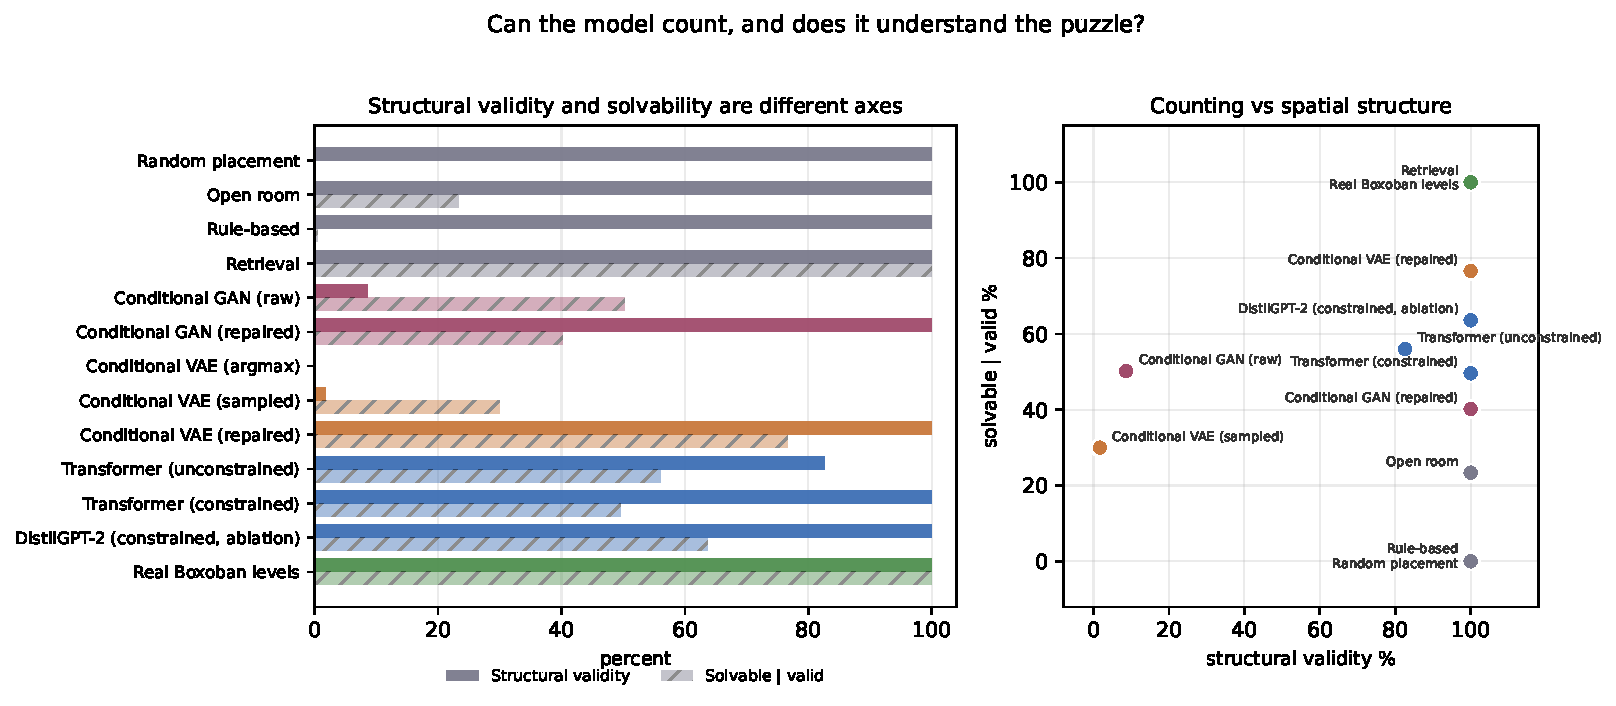
\includegraphics[width=0.86\textwidth]{../figures/fig2_validity_vs_solvability.pdf}
\caption{Left: structural validity (solid) and solvability given validity
(hatched) are different axes, and a family can be strong on one and weak on the
other. Right: the same data as a scatter. The one-shot families sit at the far
left, because they cannot count, while reaching solvability comparable to the
transformer once they are valid.}
\label{fig:money}
\end{figure*}

The main results appear in Table~\ref{tab:main}. We read them as five findings.

\subsection{Autoregressive models can count; one-shot decoders cannot}
The counting gap is the largest effect in the table, and it is structural rather
than a matter of capacity. The transformer reaches $82.6\%$ [$80.2$, $84.8$]
structural validity with no constraint at all, needing $1{,}024$ draws to yield
$500$ valid levels. The conditional VAE under argmax decoding yields
\textbf{zero} valid levels in $100{,}000$ draws. Sampling the VAE per cell
instead of taking the argmax raises validity only to $1.7\%$ [$1.6$, $1.9$],
requiring $29{,}184$ draws; the GAN reaches $8.6\%$.

Figure~\ref{fig:tiles} shows why, more convincingly than any percentage. The
transformer's box-count distribution is a spike at four ($87.1\%$ exactly four,
mean $3.87 \pm 0.34$). The VAE under argmax has mean $1.38 \pm 1.23$ boxes and
$0.01 \pm 0.12$ goals: the per-cell argmax of a product of marginals picks floor
or wall almost everywhere, because boxes occupy $4/100$ cells and goals $4/100$.
Per-cell \emph{sampling} restores the marginal rates almost exactly, at mean
$3.95 \pm 1.72$ boxes and $4.05 \pm 1.85$ goals, but only $21.8\%$ of samples
carry exactly four boxes: the right \emph{average} number and the wrong
\emph{joint}, because the per-cell outputs are conditionally independent given
the latent.

Constrained decoding closes the gap deterministically at $100\%$ validity, and
with a very light touch: feasibility forcing fired on $25.0\%$ of levels and
supplied a mean of only $0.378$ forced tokens per level. The model had largely
learned to count unaided; forcing supplies the last box.

\subsection{Solvability does not follow from validity}
Every non-learned baseline is $100\%$ structurally valid by construction and
still nearly worthless. Random placement is solvable $0.0\%$ of the time and the
rule-based generator $0.4\%$, despite the latter enforcing floor connectivity
and placing boxes only on live squares. Interior walls are what kill them: at
the training-median density the floor becomes a maze of narrow corridors, and a
box pushed into one freezes against the walls.

The \textbf{open-room} baseline constrains how the headline number may be read.
With no interior walls at all it is solvable $23.4\%$ [$19.9$, $27.3$] of the
time. The transformer's $49.6\%$ is significantly higher ($+26.2$ points,
$z = 8.60$, $p < 10^{-16}$), so the headline is not an artifact of an easy task,
but a reader given only ``$49.6\%$ solvable'' would substantially
overestimate what has been shown. The \textbf{retrieval} baseline makes the
complementary point: $100\%$ solvable, $0\%$ novel, nearest-neighbour distance
exactly $0.00$. Solvability alone is degenerate, maximised by copying, so the
table must be read as a joint constraint over solvability, difficulty control
and novelty.

\subsection{Repair separates counting from spatial understanding}
The most surprising row is the repaired VAE. Projecting its invalid output onto
the nearest valid grid yields $76.6\%$ [$72.7$, $80.1$] solvability, well
\emph{above} the transformer's $49.6\%$, with diversity ($37.8$) close to the
real-level reference ($38.8$) and no exact copies. The repaired GAN reaches
$40.2\%$.

The VAE is not bad at Sokoban; it is bad at arithmetic. Its per-cell marginals
already encode where boxes and goals plausibly go, and repair reads them off and
places the right number of tiles at the most probable positions. What
autoregressive generation buys is the ability to satisfy a counting constraint
\emph{while sampling}, not a better model of spatial structure, a result that
merging validity and solvability into one number would have hidden entirely.

A second, smaller inversion points the same way: the \emph{unconstrained}
transformer is more solvable given validity ($56.0\%$) than the constrained one
($49.6\%$; $z = -2.03$, $p = 0.043$). Unconstrained sampling keeps only the
$82.6\%$ of levels the model got right unaided, which are its more typical and
more solvable outputs; constrained decoding additionally rescues the levels it
would have botched, and those are worse levels. This is the distribution shift
predicted in Section~\ref{sec:constrained} appearing as a measurable cost, and
it is why both rows are reported. On the overall rate, solvable out of all
samples drawn, constrained decoding still wins, $49.6\%$ against $46.3\%$.

\subsection{Controllability splits along a predictable line}
Control is reported per attribute, never as one number, and the split is sharp.
The transformer hits the caption's wall-density bin $88.8\%$ of the time,
connectivity $80.0\%$ and box clustering $76.3\%$, against a $50\%$ chance rate
confirmed by two unconditioned controls (real levels score $48.8\%$, $53.2\%$
and $52.2\%$). But difficulty, the binned solution length, is hit only
$43.3\%$ of the time against a $33\%$ chance rate, and the rank correlation
between requested and achieved solution length is $\rho = 0.484$.

The dividing line is the one we predicted before running the experiment. Wall
density, connectivity and clustering are computable directly from the grid, so a
model that reproduces surface statistics gets them nearly for free. Solution
length is not computable without search. It is the only conditioned attribute
that requires the model to have learned something about the puzzle rather than
about its pixels, and it is the one the model controls worst.

That correlation is also \textbf{censored}: $55.2\%$ of suite samples have no
achieved length, because they were proven unsolvable, and the surviving
subsample is biased toward easy levels, the direction that inflates $\rho$.
The honest reading is that $0.484$ is an upper bound on a weak effect.

\subsection{Seed variance is large, and it bounds what can be claimed}
\label{sec:seeds}
We trained the primary transformer configuration three times, changing only the
seed, and sampled and solved each identically. Structural validity is perfectly
stable at $100.0\% \pm 0.0$, unsurprisingly, since constrained decoding
guarantees it, and diversity is stable at $38.60 \pm 0.31$. But
solvability-given-validity is \textbf{not}: $46.6\%$, $34.6\%$ and $47.0\%$,
giving $42.7\% \pm 7.0$. Validation loss barely moves across the same three runs
($0.357 \pm 0.005$), so validation loss is a poor predictor of the quantity we
actually care about.

This number governs how firmly the rest of the table can be read, and we prefer
to state it plainly rather than lean on a single favourable run:

\begin{itemize}
\item The comparison against the baselines survives easily. Even the worst of
      the three seeds ($34.6\%$) is far above open room ($23.4\%$) and
      rule-based ($0.4\%$).
\item The comparison against DistilGPT-2 also survives, but only because we
      retrained that model three times as well rather than trusting its single
      run (Section~\ref{sec:pretrain}).
\item The constrained-versus-unconstrained gap ($6.4$ points) is smaller than
      the seed spread. It is a within-checkpoint decoding comparison, so
      training-seed variance does not apply to it directly, but it is measured
      on one model and should be treated as indicative.
\end{itemize}

Every remaining row in this paper is single-seed and its caption says so. Given
a $\pm 7$ point spread on the headline metric, no row-to-row difference under
about $15$ points should be read as established without repeated runs.

\subsection{Pretraining transfers across a vocabulary boundary}
\label{sec:pretrain}
The DistilGPT-2 ablation discards the $50257 \times 768$ embedding matrix and
the tied LM head and re-initialises both for our $48$-symbol vocabulary, so
nothing lexical can transfer: only the attention and MLP blocks survive.
Because the from-scratch model's own seed spread is $\pm 7.0$ points, a
single-run comparison would prove nothing, so we trained the ablation three
times as well.

Across three seeds it reaches $\mathbf{64.2\% \pm 1.8}$ solvability against the
from-scratch model's $42.7\% \pm 7.0$, a $21.5$-point gap. The two sets of
runs do not overlap at all ($62.8$--$66.2$ against $34.6$--$47.0$), which is the
strongest separation obtainable from three runs per arm: the exact permutation
test returns $p = 0.05$, its floor at this sample size, and a Welch $t$-test
gives $t = 5.12$, $p = 0.028$. It also needs less rescuing from the constrained
decoder ($10.0\% \pm 3.4$ of levels against $33.7\% \pm 18.9$) and controls
solution length better ($\rho = 0.673$ against $0.484$). Pretrained
sequence-modelling machinery therefore does transfer to a domain that shares no
vocabulary with the pretraining corpus.

A second, unplanned observation is arguably more interesting than the mean
shift: the pretrained model is far more \textbf{stable} across seeds, with a
standard deviation of $1.8$ points against $7.0$, a $4.0\times$ reduction. We
flag this as an observation rather than a result: with three runs per arm a
variance test has almost no power, and Levene's test is unsurprisingly
inconclusive ($p = 0.50$). If it holds up at larger $n$, it would suggest that
what pretraining buys in this setting is partly a better-conditioned
initialisation rather than transferred knowledge, which would be worth
separating.

The cost is unambiguous: $4.0\times$ the parameters ($43.4$M against $10.7$M)
and $6.8\times$ the training time ($3897$\,s against $573$\,s, averaged over the
same three runs).

\subsection{Temperature trades solvability against diversity}
Figure~\ref{fig:pareto} shows a clean monotone trade-off: solvability falls from
$61.2\%$ at $T = 0.6$ to $34.8\%$ at $T = 1.5$, while diversity rises from
$35.8$ to a peak of $39.0$ at $T = 1.2$. $T = 1.5$ is Pareto-dominated: it
loses solvability without buying diversity back. At $T = 1.0$ the model already
matches the real-level diversity reference ($38.9$ against $38.8$).

\begin{figure*}[!tb]
\centering
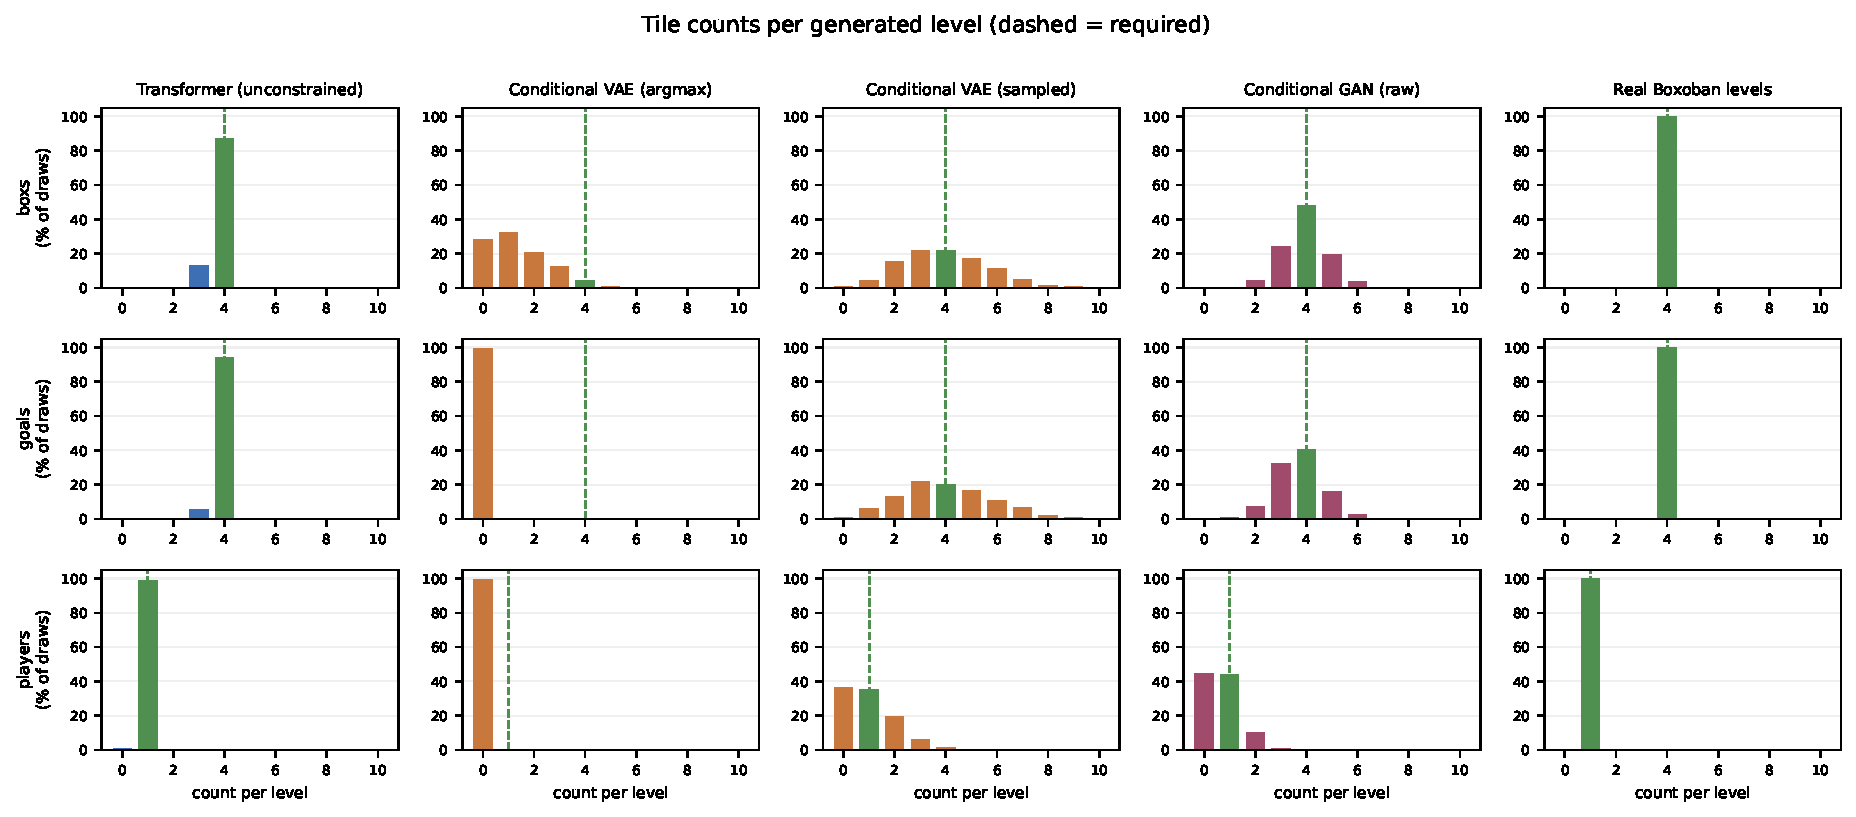
\includegraphics[width=0.88\textwidth]{../figures/fig3_tile_counts.pdf}
\caption{Tile counts per generated level over raw draws, valid or not. The
dashed line marks the required count. The transformer's distribution is a spike
at four; the VAE under argmax collapses to a near-empty room; VAE sampling
recovers the right marginal rate with the wrong joint.}
\label{fig:tiles}
\end{figure*}

\begin{figure}[!tb]
\centering
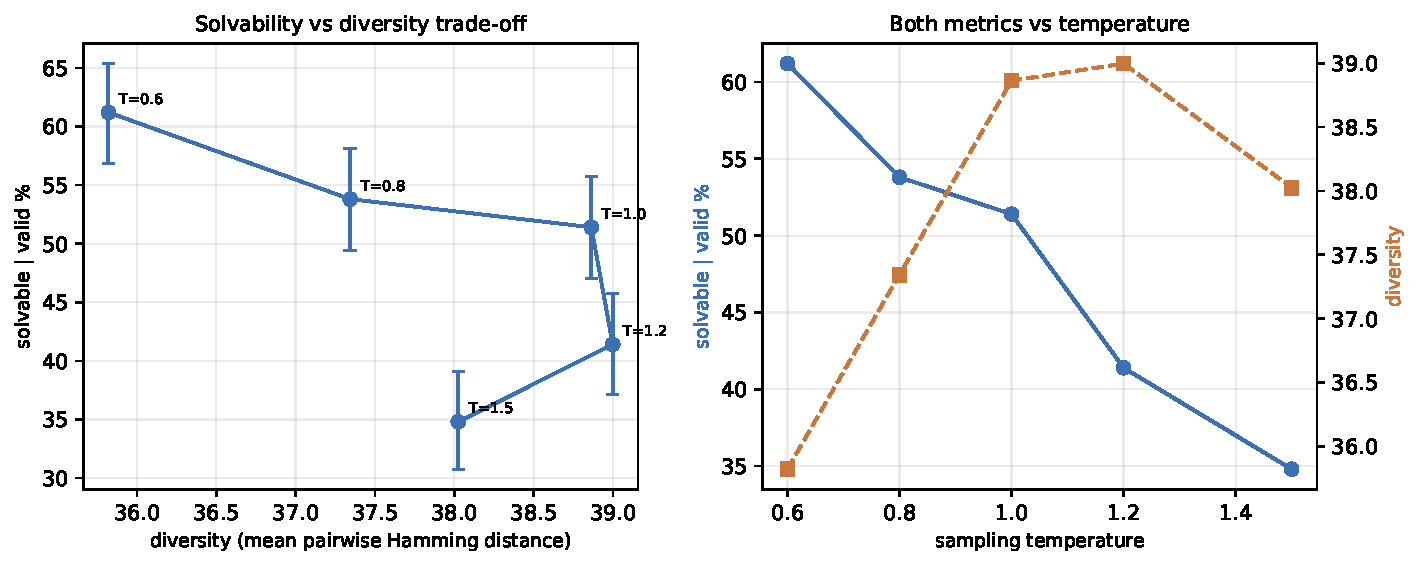
\includegraphics[width=0.98\columnwidth]{../figures/fig5_temperature_pareto.pdf}
\caption{Solvability against diversity for the constrained transformer across
sampling temperatures. Bars are Wilson 95\% intervals.}
\label{fig:pareto}
\end{figure}



\section{Failure Analysis}
\paragraph{Extrapolation fails completely}
The out-of-distribution suite requests solution lengths of $90$, $110$ and $150$
moves, against a training distribution whose $99$th percentile is $67$ and whose
maximum is $130$. Every family ignores the request. The constrained transformer
produces levels averaging $29.5$ achieved moves when asked for $115.8$, with a
rank correlation of $-0.394$; the repaired VAE averages $42.3$. Real Boxoban
levels sampled against the same captions average $30.3$, which is the correct
null, since they are not conditioned at all. Models reproduce the training length
distribution regardless of what the caption asks. Length conditioning learned
in-distribution does not extend past the data.

\paragraph{The one-shot failure mode is a plausible, empty room}
The VAE's argmax output is not noise. It is a clean, empty, unplayable room with
roughly one box and no goals whatsoever. It fails the constraint in the most
systematic way available, and it fails \emph{silently}: nothing about the output
looks malformed, there is simply no puzzle in it. A soft metric comparing tile
histograms in aggregate would not obviously flag this, which is a small argument
for verification over proxies.

\paragraph{Hand-written domain knowledge is not a shortcut}
The rule-based generator, with connectivity checks plus live-square placement,
achieves $0.4\%$ solvability, \emph{worse} than an empty room. We checked two
alternative explanations before accepting that number. It is not an unsound
prune: re-solving $450$ baseline levels with deadlock pruning disabled at a
$10\times$ node cap gives identical verdicts. And it is not caused by starting
in a deadlock: additionally rejecting frozen start states moves the rate by less
than one point. The levels die after the first push, not before it. Real Boxoban
levels reach $100\%$ at the same wall density only because they are built by
reverse play from an already-solved state, which is a fundamentally different
construction from sampling walls and then dropping boxes onto them.

\section{Limitations}

\begin{itemize}
\item \textbf{Constrained decoding shifts the sampling distribution.}
      Mask-then-renormalise at each step does not sample from the model's
      distribution conditioned on the valid set; it is a greedy local
      approximation to it.
\item \textbf{Conditioning channels differ across families.} The transformer is
      conditioned on caption text and the one-shot models on a $10$-dimensional
      vector, so the comparison is not perfectly controlled on conditioning.
\item \textbf{Reconstructed move length is an upper bound}, quantified in
      Section~\ref{sec:solver} at $+40.5\%$ mean excess. We avoid it where it
      matters by using exact move-optimal search for controllability.
\item \textbf{A single game at a single fixed size}: $10\times10$, four boxes,
      four goals. Nothing here shows the finding generalises to other tile games
      or other grid sizes.
\item \textbf{Large seed variance.} The transformer and the DistilGPT-2
      ablation were each run with three seeds; the transformer's solvability
      spread is $\pm 7.0$ points (Section~\ref{sec:seeds}). Every remaining row
      (the VAE, the GAN and all baselines) is a single run, and
      differences smaller than roughly $15$ points between those rows are not
      established. Three runs per arm is also too few to test the variance
      reduction we observed under pretraining.
\item \textbf{Untuned hyperparameters.} Learning rate, batch size and epoch count
      were chosen once and never swept, for any model (Tier 3). We did not try
      $1\mathrm{e}{-4}$ before settling on $3\mathrm{e}{-4}$.
\item \textbf{Inverse-binomial sampling.} Because we draw until $500$ valid
      levels are collected, structural-validity intervals are close
      approximations rather than exact fixed-$n$ binomial intervals.
\item \textbf{Censored controllability.} Achieved solution length exists only for
      solved levels, so the length correlation is computed on a subsample biased
      toward easy levels. We report the censoring rate alongside it.
\end{itemize}

\section{Ethics}

The models generate puzzle layouts for a single game. They consume no personal
data, produce no text about people, and inform no decisions about people. The
Boxoban corpus is procedurally generated and contains no human-authored or
personal content.

The one substantive risk is misreading the verification claim.
"Solver-verified" is a strong guarantee \emph{only} within stated bounds: a
$10\times10$ grid, four boxes, a $200{,}000$-node cap and a $10$-second
wall-clock cap. Outside them a timeout proves nothing, which is why timeouts are
a separate column rather than folded into "unsolvable". Presenting a bounded
decision procedure as an unbounded guarantee is the failure mode to avoid.

\section{Conclusion}
We evaluated three generative model families using an exhaustive A* solver as a
decision procedure rather than a proxy, reporting solved, proven-unsolvable and
timed-out separately, on a solver validated first: $100.00\%$ solve rate on
$1{,}000$ real levels, zero false proofs of unsolvability, and zero verdict
disagreements in a soundness ablation across four level distributions.

Three claims hold. Autoregressive generation satisfies counting constraints that
one-shot decoders cannot ($82.6\%$ validity unaided against \emph{zero} valid
levels in $100{,}000$ VAE draws). Solvability does not follow from validity, and
the open-room baseline at $23.4\%$ bounds how much of a headline number comes
from the task rather than the model. And the two axes come apart the other way
as well: once its counting errors are repaired the VAE is \emph{more} solvable
than the transformer, locating the autoregressive advantage in counting rather
than in spatial understanding.

Measuring across seeds proved essential. Solvability moves by $\pm 7.0$ points
across three runs of one configuration while validation loss moves by
$\pm 0.005$, so validation loss is a poor proxy for the evaluated property.
Repeating the pretraining ablation under the same protocol settles it:
$64.2\% \pm 1.8$ against $42.7\% \pm 7.0$, with no overlap between the two sets
of runs, so pretrained sequence-modelling machinery transfers even when no
vocabulary does.

The most interesting negative result is the controllability split. Attributes
computable from the grid are controlled well; solution length, which requires
search to evaluate, is controlled weakly ($\rho = 0.484$, censored) and not at
all out of distribution. A model conditioned on ``hard'' learns what hard levels
\emph{look like}, not what makes them hard, and that gap is invisible to any
metric that does not run the game.

\section*{Reproducibility}

All code, configurations, checkpoints, generated levels with per-level solver
verdicts and result JSON artifacts are released, along with four further figures
kept out of the paper for space: the pipeline schematic, a qualitative grid of
generated levels for every family, the node-cap sensitivity curve and the VAE
latent interpolation. Every artifact embeds its
configuration, seed and git commit; every table here is regenerated from them by
one command, and a checked-in script re-derives all $108$ numbers quoted in the
prose from the same artifacts.

\bibliographystyle{IEEEtran}
\bibliography{refs}

\end{document}
